% Build with XeLaTeX (Indic scripts): xelatex main && bibtex main && xelatex main && xelatex main
% Overleaf: Menu > Compiler > XeLaTeX.  acl.sty and acl_natbib.bst are the unmodified official ACL style files.
\documentclass[11pt]{article}

% `preprint' is the official ACL option that shows author names and affiliations (the demo track is single-blind).
\usepackage[preprint]{acl}
\usepackage{microtype}
\usepackage[english,bidi=default]{babel}
\babelfont{rm}{TeXGyreTermesX}
\usepackage{fontspec}
% Noto Sans Devanagari / Gujarati are bundled in fonts/ (SIL OFL 1.1), so the build needs no system fonts for Indic text.
\newfontfamily\hifont[Path=fonts/,Extension=.ttf,UprightFont=NotoSansDevanagari-Regular,BoldFont=NotoSansDevanagari-Bold,Script=Devanagari]{NotoSansDevanagari}
\newfontfamily\gufont[Path=fonts/,Extension=.ttf,UprightFont=NotoSansGujarati-Regular,BoldFont=NotoSansGujarati-Bold,Script=Gujarati]{NotoSansGujarati}
\newcommand{\hi}[1]{{\hifont #1}}   % Hindi and Marathi (Devanagari)
\newcommand{\gu}[1]{{\gufont #1}}   % Gujarati

\usepackage{booktabs,graphicx,amsmath,array,multirow,xcolor,enumitem,float}
\setlist{nosep,leftmargin=*}
\setcounter{topnumber}{3}\setcounter{bottomnumber}{2}\setcounter{totalnumber}{5}\setcounter{dbltopnumber}{3}
\renewcommand{\topfraction}{0.9}\renewcommand{\bottomfraction}{0.8}\renewcommand{\textfraction}{0.08}
\renewcommand{\floatpagefraction}{0.75}\renewcommand{\dblfloatpagefraction}{0.75}
\newcolumntype{L}[1]{>{\raggedright\arraybackslash}p{#1}}

\newcommand{\sys}{Indic AAC Studio}
\newcommand{\nstated}{\textit{n.s.}}
\newcommand{\cn}[1]{\raisebox{.15ex}{\textcircled{\scriptsize #1}}}   % numbered callout used in Figure 2
% Release location of the reviewer package (source, fixtures, scorer, raw outputs, screencast): AUTHORS MUST SET THIS to a public (or anonymized) URL before submission.
\newcommand{\demourl}{\url{https://github.com/speechforge/AAC_System}}
% Code license named in the Availability section: AUTHORS MUST CONFIRM and add the matching license file to the release.
\newcommand{\codelicense}{Apache License 2.0}
% Required concept instances in the primary set: the denominator of the Kept column of Table 2.
\newcommand{\NConc}{215}

% Every number in the text is regenerated from the evaluation result files; only two caption/label strings of the generated tables were edited by hand in v2 (no number was changed).
% AUTO-GENERATED by eval/make_tex.py from eval/results/*.json -- do not edit
\newcommand{\NScen}{184}
\newcommand{\NScenCM}{8}
\newcommand{\NOverlap}{9}
\newcommand{\NPrimEN}{46}
\newcommand{\NAllEN}{46}
\newcommand{\NPrimHI}{45}
\newcommand{\NAllHI}{46}
\newcommand{\NPrimGU}{42}
\newcommand{\NAllGU}{46}
\newcommand{\NPrimMR}{42}
\newcommand{\NAllMR}{46}
\newcommand{\NPrimAll}{175}
\newcommand{\PDNEN}{\mbox{+43\,pp [+28, +59]}}
\newcommand{\CDNEN}{22/46\,vs\,2/46}
\newcommand{\PDNHI}{\mbox{+67\,pp [+53, +80]}}
\newcommand{\CDNHI}{31/45\,vs\,1/45}
\newcommand{\PDNGU}{\mbox{+40\,pp [+24, +57]}}
\newcommand{\CDNGU}{21/42\,vs\,4/42}
\newcommand{\PDNMR}{\mbox{+52\,pp [+36, +69]}}
\newcommand{\CDNMR}{23/42\,vs\,1/42}
\newcommand{\PDTEN}{\mbox{\ensuremath{-}24\,pp [\ensuremath{-}37, \ensuremath{-}13]}}
\newcommand{\CDTEN}{22/46\,vs\,33/46}
\newcommand{\PDTHI}{\mbox{+0\,pp [+0, +0]}}
\newcommand{\CDTHI}{31/45\,vs\,31/45}
\newcommand{\PDTGU}{\mbox{\ensuremath{-}14\,pp [\ensuremath{-}26, \ensuremath{-}5]}}
\newcommand{\CDTGU}{21/42\,vs\,27/42}
\newcommand{\PDTMR}{\mbox{\ensuremath{-}10\,pp [\ensuremath{-}21, +0]}}
\newcommand{\CDTMR}{23/42\,vs\,27/42}
\newcommand{\PDPEN}{\mbox{+41\,pp [+26, +57]}}
\newcommand{\CDPEN}{22/46\,vs\,3/46}
\newcommand{\PDPHI}{\mbox{+16\,pp [+7, +27]}}
\newcommand{\CDPHI}{31/45\,vs\,24/45}
\newcommand{\PDPGU}{\mbox{+2\,pp [+0, +7]}}
\newcommand{\CDPGU}{21/42\,vs\,20/42}
\newcommand{\PDPMR}{\mbox{+12\,pp [+2, +24]}}
\newcommand{\CDPMR}{23/42\,vs\,18/42}
\newcommand{\PSUEN}{\mbox{+24\,pp [+13, +37]}}
\newcommand{\CSUEN}{33/46\,vs\,22/46}
\newcommand{\PSUHI}{\mbox{+22\,pp [+11, +36]}}
\newcommand{\CSUHI}{41/45\,vs\,31/45}
\newcommand{\PSUGU}{\mbox{+12\,pp [+2, +21]}}
\newcommand{\CSUGU}{26/42\,vs\,21/42}
\newcommand{\PSUMR}{\mbox{+21\,pp [+7, +36]}}
\newcommand{\CSUMR}{32/42\,vs\,23/42}
\newcommand{\PSTEN}{\mbox{\ensuremath{-}28\,pp [\ensuremath{-}41, \ensuremath{-}15]}}
\newcommand{\CSTEN}{33/46\,vs\,46/46}
\newcommand{\PSTHI}{\mbox{\ensuremath{-}9\,pp [\ensuremath{-}18, \ensuremath{-}2]}}
\newcommand{\CSTHI}{41/45\,vs\,45/45}
\newcommand{\PSTGU}{\mbox{\ensuremath{-}19\,pp [\ensuremath{-}31, \ensuremath{-}7]}}
\newcommand{\CSTGU}{26/42\,vs\,34/42}
\newcommand{\PSTMR}{\mbox{\ensuremath{-}24\,pp [\ensuremath{-}38, \ensuremath{-}12]}}
\newcommand{\CSTMR}{32/42\,vs\,42/42}
\newcommand{\PSPEN}{\mbox{+61\,pp [+46, +74]}}
\newcommand{\CSPEN}{33/46\,vs\,5/46}
\newcommand{\PSPHI}{\mbox{+33\,pp [+20, +47]}}
\newcommand{\CSPHI}{41/45\,vs\,26/45}
\newcommand{\PSPGU}{\mbox{+24\,pp [+12, +38]}}
\newcommand{\CSPGU}{26/42\,vs\,16/42}
\newcommand{\PSPMR}{\mbox{+19\,pp [+7, +31]}}
\newcommand{\CSPMR}{32/42\,vs\,24/42}
\newcommand{\PLLEN}{\mbox{\ensuremath{-}4\,pp [\ensuremath{-}11, +0]}}
\newcommand{\CLLEN}{1/46\,vs\,3/46}
\newcommand{\PLLHI}{\mbox{+0\,pp [+0, +0]}}
\newcommand{\CLLHI}{24/45\,vs\,24/45}
\newcommand{\PLLGU}{\mbox{+0\,pp [+0, +0]}}
\newcommand{\CLLGU}{20/42\,vs\,20/42}
\newcommand{\PLLMR}{\mbox{+0\,pp [+0, +0]}}
\newcommand{\CLLMR}{18/42\,vs\,18/42}
\newcommand{\FBUAll}{61/184}
\newcommand{\FBUEN}{30/46}
\newcommand{\FBpctUEN}{65\%}
\newcommand{\ErrUEN}{0}
\newcommand{\FBUHI}{8/46}
\newcommand{\FBpctUHI}{17\%}
\newcommand{\ErrUHI}{0}
\newcommand{\FBUGU}{6/46}
\newcommand{\FBpctUGU}{13\%}
\newcommand{\ErrUGU}{0}
\newcommand{\FBUMR}{17/46}
\newcommand{\FBpctUMR}{37\%}
\newcommand{\ErrUMR}{0}
\newcommand{\FBSAll}{67/184}
\newcommand{\FBSEN}{28/46}
\newcommand{\FBpctSEN}{61\%}
\newcommand{\ErrSEN}{0}
\newcommand{\FBSHI}{15/46}
\newcommand{\FBpctSHI}{33\%}
\newcommand{\ErrSHI}{0}
\newcommand{\FBSGU}{16/46}
\newcommand{\FBpctSGU}{35\%}
\newcommand{\ErrSGU}{0}
\newcommand{\FBSMR}{8/46}
\newcommand{\FBpctSMR}{17\%}
\newcommand{\ErrSMR}{0}
\newcommand{\LatAllEN}{11.75\,s (p90 12.75, n=69)}
\newcommand{\LatAcceptedEN}{6.05\,s (p90 6.23, n=22)}
\newcommand{\LatFallbackEN}{12.04\,s (p90 12.81, n=47)}
\newcommand{\LatAllHI}{9.97\,s (p90 18.85, n=70)}
\newcommand{\LatAcceptedHI}{9.75\,s (p90 10.08, n=52)}
\newcommand{\LatFallbackHI}{18.76\,s (p90 20.12, n=18)}
\newcommand{\LatAllGU}{7.5\,s (p90 14.77, n=72)}
\newcommand{\LatAcceptedGU}{7.45\,s (p90 7.58, n=51)}
\newcommand{\LatFallbackGU}{14.73\,s (p90 15.06, n=21)}
\newcommand{\LatAllMR}{6.58\,s (p90 13.05, n=72)}
\newcommand{\LatAcceptedMR}{6.51\,s (p90 7.06, n=49)}
\newcommand{\LatFallbackMR}{13.0\,s (p90 13.81, n=23)}
\newcommand{\LatMedAccEN}{6.05}
\newcommand{\LatMedFbEN}{12.04}
\newcommand{\LatMedAccHI}{9.75}
\newcommand{\LatMedFbHI}{18.76}
\newcommand{\LatMedAccGU}{7.45}
\newcommand{\LatMedFbGU}{14.73}
\newcommand{\LatMedAccMR}{6.51}
\newcommand{\LatMedFbMR}{13.0}
\newcommand{\LatFbMin}{12.04}
\newcommand{\LatFbMax}{18.76}
\newcommand{\NUniqueReq}{283}
\newcommand{\StageLlmOne}{1.87}
\newcommand{\StageLlmTwo}{0.0}
\newcommand{\StageLlmThree}{4.63}
\newcommand{\StageSem}{0.0}
\newcommand{\StageTts}{0.0}
\newcommand{\StageTotal}{9.46}
\newcommand{\PredENOneInf}{17.2}
\newcommand{\PredENOneTri}{16.0}
\newcommand{\PredENFiveInf}{33.4}
\newcommand{\PredENFiveTri}{32.8}
\newcommand{\PredDENOneTri}{\mbox{+1.1\,pp [+0.5, +1.8]}}
\newcommand{\PredDENFiveTri}{\mbox{+0.6\,pp [+0.0, +1.2]}}
\newcommand{\PredDENMrrTri}{\mbox{+0.007 [+0.002, +0.011]}}
\newcommand{\PredDENOneBi}{\mbox{+3.6\,pp [+2.3, +5.0]}}
\newcommand{\PredDENFiveBi}{\mbox{+3.9\,pp [+2.7, +5.1]}}
\newcommand{\PredDENMrrBi}{\mbox{+0.036 [+0.025, +0.049]}}
\newcommand{\PredDENOneUni}{\mbox{+13.5\,pp [+11.4, +15.7]}}
\newcommand{\PredDENFiveUni}{\mbox{+21.8\,pp [+19.0, +24.8]}}
\newcommand{\PredDENMrrUni}{\mbox{+0.171 [+0.148, +0.197]}}
\newcommand{\PredNEN}{2220}
\newcommand{\PredClustersEN}{60}
\newcommand{\PredOOVEN}{7.5\%}
\newcommand{\PredHIOneInf}{27.0}
\newcommand{\PredHIOneTri}{25.9}
\newcommand{\PredHIFiveInf}{44.1}
\newcommand{\PredHIFiveTri}{44.0}
\newcommand{\PredDHIOneTri}{\mbox{+1.2\,pp [+0.5, +1.9]}}
\newcommand{\PredDHIFiveTri}{\mbox{+0.1\,pp [\ensuremath{-}0.3, +0.4]}}
\newcommand{\PredDHIMrrTri}{\mbox{+0.008 [+0.004, +0.013]}}
\newcommand{\PredDHIOneBi}{\mbox{+3.0\,pp [+1.8, +4.3]}}
\newcommand{\PredDHIFiveBi}{\mbox{+1.0\,pp [+0.1, +1.9]}}
\newcommand{\PredDHIMrrBi}{\mbox{+0.023 [+0.014, +0.032]}}
\newcommand{\PredDHIOneUni}{\mbox{+20.6\,pp [+18.4, +23.0]}}
\newcommand{\PredDHIFiveUni}{\mbox{+29.5\,pp [+26.8, +32.4]}}
\newcommand{\PredDHIMrrUni}{\mbox{+0.243 [+0.220, +0.267]}}
\newcommand{\PredNHI}{2437}
\newcommand{\PredClustersHI}{60}
\newcommand{\PredOOVHI}{5.5\%}
\newcommand{\UIFalseNeg}{3}
\newcommand{\UISingle}{276}
\newcommand{\UIFeelReq}{27}
\newcommand{\GateAccU}{116}
\newcommand{\GateAccOkU}{57}
\newcommand{\GateAccPctU}{49\%}
\newcommand{\GateFbU}{59}
\newcommand{\GateFbOkU}{40}
\newcommand{\GateFbPctU}{68\%}
\newcommand{\GateAccS}{108}
\newcommand{\GateAccOkS}{71}
\newcommand{\GateAccPctS}{66\%}
\newcommand{\GateFbS}{67}
\newcommand{\GateFbOkS}{61}
\newcommand{\GateFbPctS}{91\%}
\newcommand{\CMSuccNaive}{0/8}
\newcommand{\CMSuccPre}{0/8}
\newcommand{\CMSuccDepU}{4/8}
\newcommand{\CMSuccDepS}{5/8}
\newcommand{\CMSuccTmplU}{6/8}
\newcommand{\CMSuccTmplS}{8/8}
\newcommand{\ActWrongUEN}{12/46}
\newcommand{\SuccEffUEN}{22/46}
\newcommand{\ActWrongSEN}{2/46}
\newcommand{\SuccEffSEN}{33/46}
\newcommand{\ActWrongUHI}{14/45}
\newcommand{\SuccEffUHI}{31/45}
\newcommand{\ActWrongSHI}{4/45}
\newcommand{\SuccEffSHI}{41/45}
\newcommand{\ActWrongUGU}{11/42}
\newcommand{\SuccEffUGU}{21/42}
\newcommand{\ActWrongSGU}{2/42}
\newcommand{\SuccEffSGU}{26/42}
\newcommand{\ActWrongUMR}{17/42}
\newcommand{\SuccEffUMR}{23/42}
\newcommand{\ActWrongSMR}{9/42}
\newcommand{\SuccEffSMR}{32/42}
\newcommand{\GutHitOne}{6.7}
\newcommand{\HiHmmHitOne}{24.5}
\newcommand{\CPzeroPol}{2.1\%}
\newcommand{\CPallConcept}{98.3\%}
\newcommand{\SuccNaive}{8/175}
\newcommand{\SuccPctNaive}{5\%}
\newcommand{\KeptNaive}{199/215}
\newcommand{\KeptPctNaive}{93\%}
\newcommand{\PolErrNaive}{2/175}
\newcommand{\ActWrongNaive}{3/175}
\newcommand{\AddedNaive}{7/175}
\newcommand{\OffNaive}{16/175}
\newcommand{\SuccPre}{65/175}
\newcommand{\SuccPctPre}{37\%}
\newcommand{\KeptPre}{175/215}
\newcommand{\KeptPctPre}{81\%}
\newcommand{\PolErrPre}{2/175}
\newcommand{\ActWrongPre}{54/175}
\newcommand{\AddedPre}{25/175}
\newcommand{\OffPre}{19/175}
\newcommand{\SuccDepU}{97/175}
\newcommand{\SuccPctDepU}{55\%}
\newcommand{\KeptDepU}{215/215}
\newcommand{\KeptPctDepU}{100\%}
\newcommand{\PolErrDepU}{0/175}
\newcommand{\ActWrongDepU}{54/175}
\newcommand{\AddedDepU}{4/175}
\newcommand{\OffDepU}{10/175}
\newcommand{\SuccDepS}{132/175}
\newcommand{\SuccPctDepS}{75\%}
\newcommand{\KeptDepS}{215/215}
\newcommand{\KeptPctDepS}{100\%}
\newcommand{\PolErrDepS}{0/175}
\newcommand{\ActWrongDepS}{17/175}
\newcommand{\AddedDepS}{3/175}
\newcommand{\OffDepS}{9/175}
\newcommand{\SuccTmplS}{167/175}
\newcommand{\SuccPctTmplS}{95\%}
\newcommand{\KeptTmplS}{215/215}
\newcommand{\KeptPctTmplS}{100\%}
\newcommand{\PolErrTmplS}{0/175}
\newcommand{\ActWrongTmplS}{0/175}
\newcommand{\AddedTmplS}{0/175}
\newcommand{\OffTmplS}{0/175}
\newcommand{\SuccTmplU}{118/175}
\newcommand{\SuccPctTmplU}{67\%}
\newcommand{\KeptTmplU}{215/215}
\newcommand{\KeptPctTmplU}{100\%}
\newcommand{\PolErrTmplU}{0/175}
\newcommand{\ActWrongTmplU}{57/175}
\newcommand{\AddedTmplU}{0/175}
\newcommand{\OffTmplU}{0/175}
\newcommand{\SuccLit}{0/175}
\newcommand{\SuccPctLit}{0\%}
\newcommand{\KeptLit}{215/215}
\newcommand{\KeptPctLit}{100\%}
\newcommand{\PolErrLit}{0/175}
\newcommand{\ActWrongLit}{0/175}
\newcommand{\AddedLit}{0/175}
\newcommand{\OffLit}{0/175}
\newcommand{\RefARules}{384/384}
\newcommand{\RefARulesPct}{100.0\%}
\newcommand{\RefAModel}{378/384}
\newcommand{\RefAModelPct}{98.4\%}
\newcommand{\RefAHybrid}{384/384}
\newcommand{\RefAHybridPct}{100.0\%}
\newcommand{\RefARaw}{0/384}
\newcommand{\RefARawPct}{0.0\%}
\newcommand{\RefALat}{31.8}
\newcommand{\RefFRules}{384/384}
\newcommand{\RefFRulesPct}{100.0\%}
\newcommand{\RefFModel}{379/384}
\newcommand{\RefFModelPct}{98.7\%}
\newcommand{\RefFHybrid}{384/384}
\newcommand{\RefFHybridPct}{100.0\%}
\newcommand{\RefFRaw}{0/384}
\newcommand{\RefFRawPct}{0.0\%}
\newcommand{\RefFLat}{32.2}
\newcommand{\IGSent}{15{,}505}
\newcommand{\IGTok}{112{,}875}
\newcommand{\IGDepth}{181}
\newcommand{\OffReady}{10.2}
\newcommand{\OffFirstEn}{13.94}
\newcommand{\OffHi}{10.1}
\newcommand{\NSymbols}{69}
\newcommand{\NCategories}{9}

% generated by make_tables.py from eval/results/*.json and scored.csv
\newcommand{\XPreSSucc}{71/175}
\newcommand{\XPreSSuccPct}{41\%}
\newcommand{\XPreSKept}{185/215}
\newcommand{\XPreSKeptPct}{86\%}
\newcommand{\XPreSPol}{36/175}
\newcommand{\XPreSWrong}{30/175}
\newcommand{\XPreSNoAct}{44/175}
\newcommand{\XPreSAdded}{21/175}
\newcommand{\XPreSOff}{17/175}
\newcommand{\XPreUSucc}{65/175}
\newcommand{\XPreUSuccPct}{37\%}
\newcommand{\XPreUKept}{175/215}
\newcommand{\XPreUKeptPct}{81\%}
\newcommand{\XPreUPol}{2/175}
\newcommand{\XPreUWrong}{54/175}
\newcommand{\XPreUNoAct}{33/175}
\newcommand{\XPreUAdded}{25/175}
\newcommand{\XPreUOff}{19/175}
\newcommand{\XDepSSucc}{132/175}
\newcommand{\XDepSSuccPct}{75\%}
\newcommand{\XDepSKept}{215/215}
\newcommand{\XDepSKeptPct}{100\%}
\newcommand{\XDepSPol}{0/175}
\newcommand{\XDepSWrong}{17/175}
\newcommand{\XDepSNoAct}{24/175}
\newcommand{\XDepSAdded}{3/175}
\newcommand{\XDepSOff}{9/175}
\newcommand{\XDepUSucc}{97/175}
\newcommand{\XDepUSuccPct}{55\%}
\newcommand{\XDepUKept}{215/215}
\newcommand{\XDepUKeptPct}{100\%}
\newcommand{\XDepUPol}{0/175}
\newcommand{\XDepUWrong}{54/175}
\newcommand{\XDepUNoAct}{21/175}
\newcommand{\XDepUAdded}{4/175}
\newcommand{\XDepUOff}{10/175}
\newcommand{\XTmplSSucc}{167/175}
\newcommand{\XTmplSSuccPct}{95\%}
\newcommand{\XTmplSKept}{215/215}
\newcommand{\XTmplSKeptPct}{100\%}
\newcommand{\XTmplSPol}{0/175}
\newcommand{\XTmplSWrong}{0/175}
\newcommand{\XTmplSNoAct}{8/175}
\newcommand{\XTmplSAdded}{0/175}
\newcommand{\XTmplSOff}{0/175}
\newcommand{\XTmplUSucc}{118/175}
\newcommand{\XTmplUSuccPct}{67\%}
\newcommand{\XTmplUKept}{215/215}
\newcommand{\XTmplUKeptPct}{100\%}
\newcommand{\XTmplUPol}{0/175}
\newcommand{\XTmplUWrong}{57/175}
\newcommand{\XTmplUNoAct}{0/175}
\newcommand{\XTmplUAdded}{0/175}
\newcommand{\XTmplUOff}{0/175}
\newcommand{\XNaiveSucc}{8/175}
\newcommand{\XNaiveSuccPct}{5\%}
\newcommand{\XNaiveKept}{199/215}
\newcommand{\XNaiveKeptPct}{93\%}
\newcommand{\XNaivePol}{2/175}
\newcommand{\XNaiveWrong}{3/175}
\newcommand{\XNaiveNoAct}{163/175}
\newcommand{\XNaiveAdded}{7/175}
\newcommand{\XNaiveOff}{16/175}
\newcommand{\XPolDropPreS}{35}
\newcommand{\XPolSpurPreS}{1}
\newcommand{\XGateAccU}{116}
\newcommand{\XGateAccPctU}{66\%}
\newcommand{\XGateFbU}{59}
\newcommand{\XGateFbPctU}{34\%}
\newcommand{\XGateOkU}{57/116}
\newcommand{\XGateOkPctU}{49\%}
\newcommand{\XFbOkU}{40/59}
\newcommand{\XFbOkPctU}{68\%}
\newcommand{\XGateAccS}{108}
\newcommand{\XGateAccPctS}{62\%}
\newcommand{\XGateFbS}{67}
\newcommand{\XGateFbPctS}{38\%}
\newcommand{\XGateOkS}{71/108}
\newcommand{\XGateOkPctS}{66\%}
\newcommand{\XFbOkS}{61/67}
\newcommand{\XFbOkPctS}{91\%}


\title{Indic AAC Studio: Concept-Gated Symbol-to-Speech Generation\\
for English, Hindi, Gujarati, and Marathi}

% Three authors: ACL's \And separates authors in a row and \AND starts a new row. The title box is enlarged (a multiple of the line height, as the official template allows) so that the two rows fit.
\setlength\titlebox{13\baselineskip}
\author{Ravindrakumar M. Purohit \\
  Speech Research Lab \\
  Dhirubhai Ambani University (DA-IICT) \\
  Gandhinagar, India
  \And
  Jaydeep Parmar \\
  Pandit Deendayal Energy \\
  University (PDEU) \\
  Gandhinagar, India
  \AND
  Hemant A. Patil \\
  Speech Research Lab, Dhirubhai Ambani University (DA-IICT), Gandhinagar, India}

\begin{document}
\maketitle
\begin{figure*}[t]
\centering
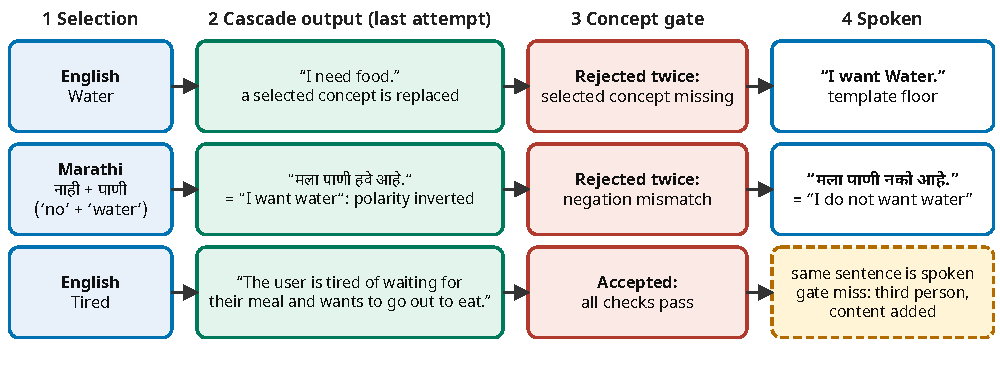
\includegraphics[width=\textwidth]{figures/teaser.pdf}
\caption{Three recorded requests from the frozen evaluation. The gate rejects a cascade output that replaces a selected concept (row~1) or inverts polarity (row~2, explicit negation field) and speaks a template built from the user's labels; it accepts a fluent third-person sentence that adds content (row~3, a miss). Marathi glosses are given in quotation marks.}
\label{fig:teaser}
\end{figure*}


\begin{abstract}
Symbol-based augmentative and alternative communication (AAC) devices voice telegraphic labels, whereas Hindi, Gujarati, and Marathi need case marking, agreement, and negation.
A language model can expand a selection into a sentence, but it can also replace a concept, drop a negation, or add content, and an AAC device speaks for its user.
We present \sys{}, a web system for English, Hindi, Gujarati, and Marathi that speaks a model-generated sentence only if a deterministic gate confirms the selected concepts, polarity, and intended act, and otherwise speaks a template built from the user's own labels.
On \NPrimAll{} frozen scenarios, the gate keeps all \NConc{} required concepts (the ungated cascade keeps \XPreUKeptPct{}--\XPreSKeptPct{}), removes its polarity errors (\XPreSPol{} with explicit intent fields), and raises success from \XPreSSuccPct{} to \XDepSSuccPct{} when intent and polarity are passed explicitly (\XPreUSuccPct{} to \XDepUSuccPct{} with the web client's inferred fields); one unconstrained prompt succeeds on \XNaiveSuccPct{}.
A template alone reaches \XTmplSSuccPct{} under explicit fields, so the gate is a safeguard and not a quality gain.
A suffix-trie predictor trained on AAC dialogues exceeds trigram backoff by 1.1 hit@1 points in English and 1.2 in Hindi.
Speech synthesis is integrated but was not evaluated; code, fixtures, scorer, and a screencast are released.
\end{abstract}

\section{Introduction}
\label{sec:intro}

A person who communicates through a symbol-based AAC board composes a message by tapping pictograms, and the device voices the selected labels.
The message is telegraphic---\emph{Water}, or \emph{No}\,+\,\emph{Pizza}---and the listener cannot see the selection.
For people who cannot rely on speech, such messages carry requests, refusals, and reports of pain, so a sentence that sounds fluent but misstates the selection can cause harm.

\paragraph{Why Indian languages need more than labels.}
India's 2011 Census recorded 26.8~million persons with disabilities, 2.21\% of the population \citep{census2011}, without isolating those who rely on AAC.
Hindi, Gujarati, and Marathi express a want with a verb-final, experiencer-dative construction: \emph{Water} becomes \hi{मुझे पानी चाहिए।} in Hindi, \gu{મને પાણી જોઈએ છે.} in Gujarati, and \hi{मला पाणी हवे आहे.} in Marathi.
Feelings and negation use other constructions, so a literal join of labels is hard for a listener to parse.
A language model can generalize across combinations, but the small model that fits a 4\,GB GPU in our setup, Qwen2.5-0.5B-Instruct, produced a successful sentence for only \XNaiveSucc{} of our scenarios when prompted without constraints (Section~\ref{sec:eval}).

\paragraph{Fluent is not faithful.}
An AAC device speaks for its user, so the sentence must preserve what was selected.
Figure~\ref{fig:teaser} shows how the cascade evaluated here fails: it replaced the concept for \emph{Water}, inverted polarity for Marathi \emph{No}\,+\,\emph{Water}, and added content for \emph{Tired}.
When negation was passed explicitly, the ungated cascade dropped or inverted polarity in \XPreSPol{} scenarios.

\paragraph{Concept-gated generation.}
\sys{} treats the selection as a contract.
A \emph{concept ledger} lists the concepts that must appear and those that must not; a prompted cascade proposes a sentence; a deterministic \emph{gate} accepts it only if the ledger is satisfied; and otherwise a template built from the user's own labels is spoken (Figure~\ref{fig:teaser}).
The model can improve phrasing but cannot change what was selected.
Qwen2.5-0.5B-Instruct and IndicF5 are used as released; our contributions are the constraint layer, the interface and trained predictors around it, and a frozen protocol that measures them against matched baselines.
The system serves symbol-board users in these four languages and the caregivers, clinicians, and researchers who configure boards.

\begin{itemize}
\item \textbf{Concept-gated realization:} a ledger, a four-part acceptance rule, a retry policy, and a template floor, behind an interface that carries intent and polarity explicitly (Section~\ref{sec:system}).
\item \textbf{A four-language demo} with a \NSymbols{}-symbol board, Quick Express phrases, personal vocabulary, voice cloning, and predictors trained on AAC dialogues and streamed text (Section~\ref{sec:system}, Appendix~\ref{app:models}).
\item \textbf{A frozen, paired evaluation} of \NPrimAll{} scenarios against literal, template, unconstrained-prompt, and pre-gate baselines: the gate keeps every selected concept and removes all polarity errors, explicit intent fields cut wrong-act outputs from \XDepUWrong{} to \XDepSWrong{}, and a template alone is a strong floor on this closed grid (Section~\ref{sec:eval}).
\end{itemize}

\section{Related Work}
\label{sec:related}

\paragraph{Expanding telegraphic input.}
Compansion expanded telegraphic AAC input into well-formed sentences with syntactic and semantic rules \citep{mccoy1998compansion}.
Recent systems apply language models to other inputs: SpeakFaster expands abbreviated text for eye-gaze typists with ALS \citep{cai2024speakfaster}; ConnecTone suggests text from conversational context and speaks it with a style-adaptive TTS \citep{francis2024connectone}; and \citet{mohan2024composition} compose messages from typed, emoji, or spoken input in the user's own voice.
\citet{karmakar-sinha-2024-aiding} propose a language-agnostic mapping between text and AAC symbols, and \citet{vertanen2026multilingual} contribute multilingual AAC text collections.
\sys{} starts from symbol selections, which give the model a small concept set whose omission or inversion can be checked.

\paragraph{Boards and voices.}
Cboard is an open-source web board that states support for 46 languages without naming Hindi, Gujarati, or Marathi \citep{cboard}; Jellow lists 24 languages including all three and offers pre-made sentences \citep{jellow}; Avaz provides regional vocabularies and predictive text \citep{avaz}, and its FreeSpeech app teaches grammar by sentence building \citep{avazfreespeech}.
\citet{francis2025static} add generated symbols and zero-shot voice cloning to a symbol board.

\paragraph{Gap.}
Table~\ref{tab:related} compares documented capabilities (\nstated{}: not stated by the source, not absent).
Among these sources, none documents a deterministic check that preserves selected concepts and polarity in model-generated Indian-language sentences on a symbol board; we make no claim about undocumented products, and Section~\ref{sec:eval} compares against matched baselines instead.

\begin{table*}[t]
\centering\footnotesize
\setlength{\tabcolsep}{4pt}
\begin{tabular}{@{}L{2.0cm}L{2.5cm}L{2.9cm}L{2.7cm}L{2.2cm}L{2.0cm}@{}}
\toprule
System & Input & Languages (as stated) & Sentence realization & Output check & Speech \\
\midrule
Cboard & symbols, text & 46; HI, GU, MR not named & \nstated & \nstated & text-to-speech \\
Jellow & symbols, keyboard & 24, incl.\ HI, MR, GU & pre-made sentences & \nstated & Google TTS \\
Avaz & symbols, keyboard & regional; list \nstated & predictive text & \nstated & \nstated \\
\citeauthor{francis2025static} & symbols (generated) & \nstated & none described & \nstated & zero-shot cloning \\
ConnecTone & speech, text & \nstated & suggestions from context & \nstated & style-adaptive TTS \\
\citeauthor{mohan2024composition} & typed, emoji, spoken & \nstated & LLM phrase suggestions & \nstated & user's own voice \\
SpeakFaster & abbreviated text (gaze) & \nstated & LLM abbreviation expansion & \nstated & \nstated \\
\midrule
\textbf{\sys{}} & symbols, text & EN, HI, GU, MR; Hinglish option & prompted Qwen cascade & concept, polarity, intent gate & IndicF5, browser speech \\
\bottomrule
\end{tabular}
\caption{Documented capabilities of the closest systems, from the cited paper or the vendor page read on 2026-11-12. \nstated{}: not stated by the source.}
\label{tab:related}
\end{table*}

\section{System Design and Demo Walkthrough}
\label{sec:system}

\begin{figure*}[t]
\centering
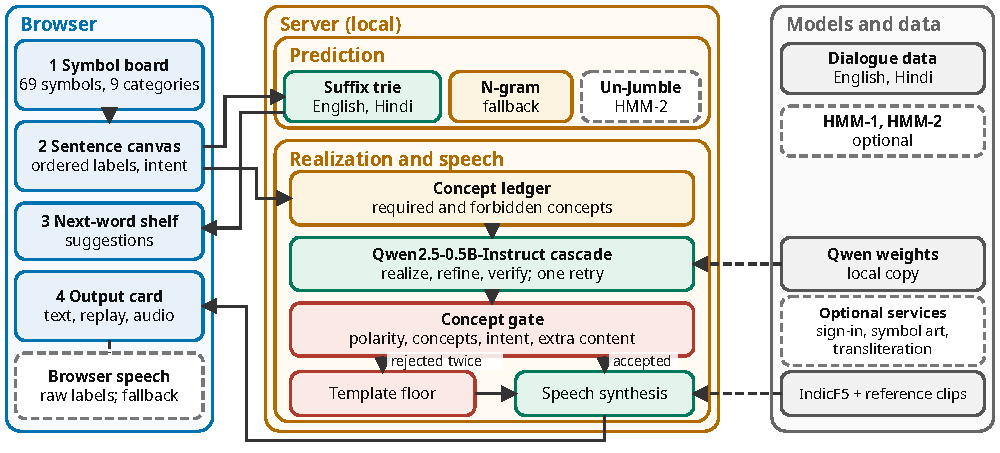
\includegraphics[width=0.92\textwidth]{figures/architecture.pdf}
\caption{Architecture of \sys{}. A selection in the browser goes to the server for next-word suggestions and for realization. The cascade output is spoken only if the gate accepts it; after two rejections a template built from the user's labels is spoken. Dashed boxes are optional components.}
\label{fig:arch}
\end{figure*}

\paragraph{Walkthrough.}
The user picks a language and taps symbols from a board of \NSymbols{} symbols in \NCategories{} categories, labeled in English, Hindi, Gujarati, and Marathi (Figure~\ref{fig:ui}, \cn{1}); free text, emoji search, and a personal ``My Words'' grid extend the vocabulary.
Selections accumulate on a sentence canvas (\cn{2}), and a shelf proposes next words with their probabilities (\cn{3}).
\emph{Speak} voices the literal labels with the browser's speech synthesis and needs no model round trip.
\emph{AI Polish \& Speak} (\cn{4}) sends the selection to the server, which returns a sentence that the output card shows while it is spoken (\cn{5}); the card offers Replay, Copy, and a bookmark for a one-tap Quick Picks shelf.
A Quick Express row speaks emergency phrases (Help, Water, Bathroom, Pain) in one tap, Un-Jumble reorders canvas words with a second HMM, and an accessibility dock adjusts card and text size, contrast, grayscale, and speech speed.

\begin{figure}[t]
\centering
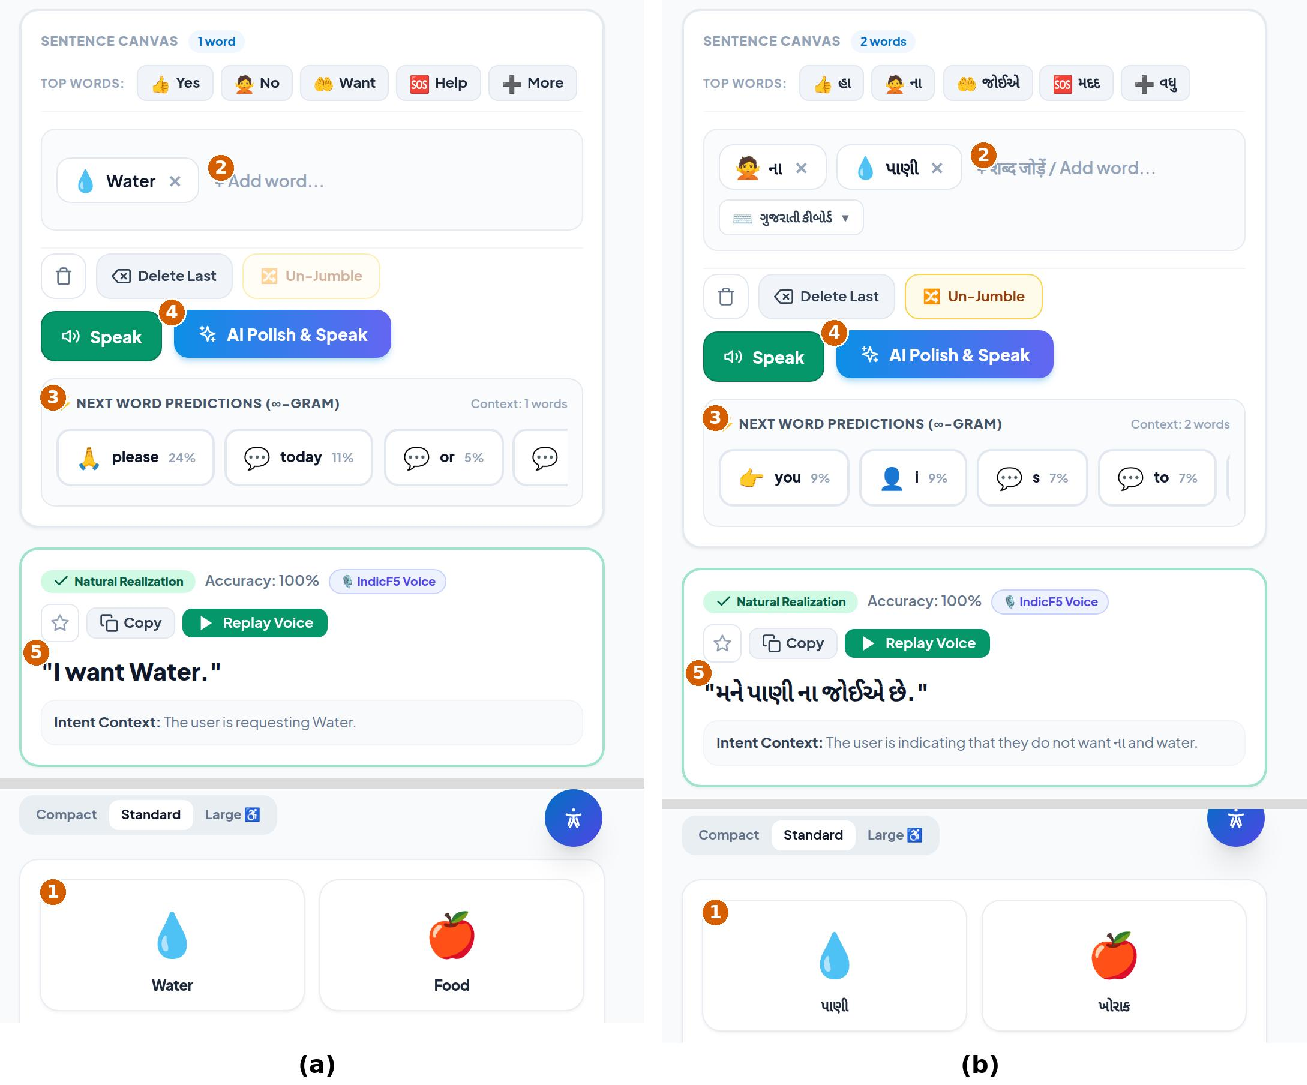
\includegraphics[width=\columnwidth]{figures/ui_panel.pdf}
\caption{The running build (Chrome, 520\,px viewport). (a)~English \emph{Water}: the cascade output was rejected and the template was spoken. (b)~Gujarati \gu{ના}\,+\,\gu{પાણી} (\emph{no}\,+\,\emph{water}): the cascade output was accepted. Callouts: \cn{1} symbol, \cn{2} canvas, \cn{3} next-word shelf, \cn{4} generate, \cn{5} output. The \emph{Accuracy} badge is the validator's heuristic score, not a gate threshold.}
\label{fig:ui}
\end{figure}

\paragraph{Request and concept ledger.}
The browser sends the ordered labels with the communicative intent (request, statement, question, or negation), a negation indicator, the language, and an optional code-mixing indicator.
The web client infers intent and negation from label substrings: negation if a label contains \emph{no}, \emph{not}, or a Hindi, Gujarati, or Marathi negator; question for question words; statement for a few feeling labels; request otherwise.
Any other client can supply both fields explicitly.
The server builds a \emph{ledger}: a required set (intent, speaker, each selected concept, negation) and a forbidden set of 21 default words for unrequested times, meals, and venues, minus any word the user selected.

\paragraph{Realization and gate.}
Three prompted stages share one frozen Qwen2.5-0.5B-Instruct \citep{qwen2025qwen25}.
The realizer writes a sentence from a few-shot prompt for Hindi, Gujarati, and Marathi (12, 9, and 9 examples; greedy decoding) and from a ledger prompt for English and code-mixed output (temperature 0.1); the refiner removes unsupported content and is skipped for Indic-script candidates; the verifier returns a verdict and a minimal rewrite.
The gate then decides.
With $\nu$ the negation indicator, $E$ the selected concepts, $F$ the forbidden set, and $y$ the candidate,
\begin{equation}
\begin{split}
\mathrm{acc}(y)={}&[\mathrm{neg}(y)=\nu]\wedge\mathrm{match}(E,y)\wedge\mathrm{intent}(y)\\
&\wedge\neg\mathrm{forbid}_F(y)\wedge\neg\mathrm{time}(y).
\end{split}
\label{eq:gate}
\end{equation}
Here \emph{neg} tests a list of English, Hindi, Gujarati, and Marathi negators; \emph{match} requires every selected concept to appear (a substring, plural, and Indic-stem test); \emph{intent} rejects ``I want'' for feeling intents and requires a question cue for questions; \emph{forbid} matches words of $F$; and \emph{time} flags time words when none was selected.
The verifier's verdict is advisory, and only the gate decides.
A rejection triggers one more cascade run, and after two rejections a language-specific template built from the selected labels (e.g., ``I want Water.'') is returned.
English and code-mixed retries resample, whereas greedy Indic retries repeat.

\paragraph{Prediction and speech.}
Next-word suggestions come from an unbounded-order suffix trie in the spirit of infini-gram \citep{liu2024infinigram}: contexts of any length are matched by suffix, and scores combine with backoff 0.4.
The trie is built in under a second at start-up from the English and Hindi AAC dialogues (\IGSent{} sentences, maximum depth \IGDepth{}); two HMMs trained on streamed text (HMM-1 for next words, HMM-2 for Un-Jumble) are optional components that the evaluated build ran without (Section~\ref{sec:limits}).
The returned sentence is synthesized by IndicF5 \citep{ai4bharat2025indicf5}, a flow-matching model of the F5-TTS family \citep{chen2025f5tts}, with a 24\,kHz Vocos vocoder \citep{siuzdak2023vocos}.
A reference clip and its exact transcript condition the voice zero-shot, so a caregiver can register a familiar voice.

\paragraph{What is trained.}
Qwen2.5-0.5B-Instruct is prompted, not fine-tuned, and IndicF5 is used as released.
We train the suffix trie and a Hindi HMM on the AAC dialogues, two HMMs on streamed English text, and an English Flan-T5 refiner (Appendix~\ref{app:models}).

\section{Evaluation}
\label{sec:eval}

We ask four questions. \textbf{RQ1}: does the gate preserve what an ungated cascade loses? \textbf{RQ2}: where do the remaining errors originate? \textbf{RQ3}: how does the pipeline compare with a deterministic template? \textbf{RQ4}: do the predictors beat n-gram baselines on held-out conversations?

\paragraph{Protocol.}
We froze \NScen{} monolingual and \NScenCM{} exploratory Hinglish scenarios before scoring any output.
Each of English, Hindi, Gujarati, and Marathi has 46 board selections: food request (10), refusal (\emph{No}\,+\,food; 10), feeling (8), negated feeling (8), action and object (6), and \emph{Help} or \emph{Call} with a person (4), with gold polarity and act fixed.
Each scenario is sent as the web client builds it (\emph{client}) and with explicit intent and negation fields (\emph{explicit}).
The server ran on one GTX~1650 (4\,GB).

\paragraph{Systems and scoring.}
We compare (i) a literal join of the labels; (ii) the same Qwen model with one unconstrained prompt (no ledger, examples, verifier, or gate); (iii) the cascade output before the gate, taken from the same response as the deployed output so that gate and fallback are isolated on identical candidates; (iv) the deployed output of the live server; and (v) the template alone.
A scenario \emph{succeeds} if the output keeps every selected concept, has the gold polarity and act, adds no unselected concept, and is a first-person sentence in the target script.
A lexical scorer written independently of the gate applies these rules (Appendix~\ref{app:scorer}).
Nine scenarios whose few-shot prompt reproduces a prompt example are excluded, leaving \NPrimAll{} (EN \NPrimEN{}, HI \NPrimHI{}, GU \NPrimGU{}, MR \NPrimMR{}).
Differences are paired by scenario with 95\% bootstrap intervals (10,000 resamples).

\begin{table*}[t]
\centering\footnotesize
\setlength{\tabcolsep}{3.2pt}
\begin{tabular}{@{}l ccccc @{\hspace{6pt}} c ccccc@{}}
\toprule
 & \multicolumn{5}{c}{Scenario success (n/N)} & \multicolumn{6}{c}{Pooled diagnostics (counts)} \\
\cmidrule(lr){2-6}\cmidrule(l){7-12}
System & EN & HI & GU & MR & All & Kept$\uparrow$ & Pol.$\downarrow$ & \shortstack{Wrong\\act$\downarrow$} & \shortstack{No\\act$\downarrow$} & Added$\downarrow$ & \shortstack{Off-\\task$\downarrow$} \\
\midrule
\multicolumn{12}{@{}l}{\emph{Payload built by the web client (intent and negation inferred from labels)}}\\
Literal join & 0/46 & 0/45 & 0/42 & 0/42 & 0/175 & 215/215 & 0 & 0 & 175 & 0 & 0 \\
Unconstrained Qwen & 2/46 & 1/45 & 4/42 & 1/42 & 8/175 & 199/215 & 2 & 3 & 163 & 7 & 16 \\
Cascade before gate & 3/46 & 24/45 & 20/42 & 18/42 & 65/175 & 175/215 & 2 & 54 & 33 & 25 & 19 \\
\textbf{\sys{} (deployed)} & \textbf{22/46} & \textbf{31/45} & \textbf{21/42} & \textbf{23/42} & \textbf{97/175} & \textbf{215/215} & \textbf{0} & \textbf{54} & \textbf{21} & \textbf{4} & \textbf{10} \\
Template floor & 33/46 & 31/45 & 27/42 & 27/42 & 118/175 & 215/215 & 0 & 57 & 0 & 0 & 0 \\
\midrule
\multicolumn{12}{@{}l}{\emph{Payload with explicit intent and negation fields}}\\
Cascade before gate & 5/46 & 26/45 & 16/42 & 24/42 & 71/175 & 185/215 & 36 & 30 & 44 & 21 & 17 \\
\textbf{\sys{} (deployed)} & \textbf{33/46} & \textbf{41/45} & \textbf{26/42} & \textbf{32/42} & \textbf{132/175} & \textbf{215/215} & \textbf{0} & \textbf{17} & \textbf{24} & \textbf{3} & \textbf{9} \\
Template floor & 46/46 & 45/45 & 34/42 & 42/42 & 167/175 & 215/215 & 0 & 0 & 8 & 0 & 0 \\
\bottomrule
\end{tabular}
\caption{Primary set (175 scenarios; EN 46, HI 45, GU 42, MR 42). Success requires every selected concept, the gold polarity and act, no added concept, and an on-task first-person sentence in the target script. Kept: required concept instances present (of 215). Pol., Wrong act, No act, Added, Off-task: scenarios (of 175) with that error; one output can have several. The literal join carries no act marker by construction.}
\label{tab:results}
\end{table*}


\paragraph{RQ1: the gate preserves what the cascade loses.}
Before the gate, the cascade keeps \XPreSKeptPct{} of required concepts when intent and polarity are explicit (\XPreUKeptPct{} under client payloads) and makes \XPreSPol{} polarity errors, \XPolDropPreS{} of them dropped negations (Table~\ref{tab:results}).
With the gate and template floor, the same requests keep all \NConc{} concepts and make no polarity error.
Success rises from \XPreSSucc{} to \XDepSSucc{} with explicit fields (paired gain \PSPEN{} in English, \PSPHI{} in Hindi, \PSPGU{} in Gujarati, \PSPMR{} in Marathi) and from \XPreUSucc{} to \XDepUSucc{} under client payloads.
Gains concentrate where a model most often drops or flips a selection: with explicit fields, refusals pass from 10/38 to 38/38 and negated feelings from 2/32 to 13/32 (Table~\ref{tab:type}).
With explicit fields the gate lets model text through on \XGateAccPctS{} of requests (\XGateAccS{}/175) and returns the template for the rest; accepted outputs are fully correct in \XGateOkS{} (\XGateOkPctS{}) and template fallbacks in \XFbOkS{} (\XFbOkPctS{}).

\paragraph{RQ2: the remaining errors are mostly about intent.}
Under client payloads, \XDepUWrong{} deployed outputs express the wrong act; explicit fields cut this to \XDepSWrong{} and raise success from \XDepUSuccPct{} to \XDepSSuccPct{} (\PSUEN{} in English to \PSUMR{} in Marathi).
The client infers \textsc{request} for \UIFeelReq{} of its 32 feeling selections, so Indic feelings become wants (\hi{मुझे गुस्सा चाहिए।}, ``I want anger''), and the gate's feeling test is an English pattern.
Two defects are independent of the model: the client's substring rule marks \UIFalseNeg{} of \UISingle{} single-symbol selections as negated (e.g., \emph{Nose}), and the template has no form for client intent \textsc{negation} and returns ``I want No Pizza.''
Accepted outputs can also add perspective or content (Figure~\ref{fig:teaser}, row~3).

\paragraph{RQ3: a template is a strong floor.}
A template echoes the selected labels, so it scores well on this closed grid: \XTmplSSucc{} (\XTmplSSuccPct{}) with explicit fields and \XTmplUSucc{} under client payloads.
It is ahead of the deployed pipeline in every language except Hindi under client payloads, where they tie (deployed minus template with explicit fields: \PSTEN{} in English, \PSTHI{} in Hindi, \PSTGU{} in Gujarati, \PSTMR{} in Marathi).
The model path adds wrong-act outputs that a template does not (\XDepSWrong{} against \XTmplSWrong{}), and the lexical criterion rewards label echo without scoring fluency, so this comparison bounds what model phrasing adds and does not measure it.
We therefore treat the template as the system's floor: the gate admits model text only when it preserves concepts and polarity, as the template does by construction.

\begin{table}[t]
\centering\footnotesize
\setlength{\tabcolsep}{3pt}
\begin{tabular}{@{}lcccccc@{}}
\toprule
 & \multicolumn{3}{c}{English} & \multicolumn{3}{c}{Hindi} \\
\cmidrule(lr){2-4}\cmidrule(l){5-7}
Model & @1 & @5 & MRR & @1 & @5 & MRR \\
\midrule
Unigram frequency & 3.6 & 11.6 & 0.069 & 6.4 & 14.5 & 0.099 \\
Bigram, backoff & 13.6 & 29.5 & 0.204 & 24.1 & 43.1 & 0.320 \\
Trigram, backoff & 16.0 & 32.8 & 0.234 & 25.9 & 44.0 & 0.334 \\
Gutenberg HMM & 6.7 & 15.5 & 0.105 & -- & -- & -- \\
Hindi AAC HMM & -- & -- & -- & 24.5 & 41.9 & 0.315 \\
\midrule
\textbf{$\infty$-gram (deployed)} & \textbf{17.2} & \textbf{33.4} & \textbf{0.240} & \textbf{27.0} & \textbf{44.1} & \textbf{0.343} \\
\bottomrule
\end{tabular}
\caption{Next-word prediction on AAC-user utterances of 60 held-out source conversations per language (2,220 English and 2,437 Hindi contexts); hit rates in \%, MRR@10. Training and test sources are disjoint; the n-gram baselines, the trie, and the Hindi HMM share the training split, and the Gutenberg HMM is trained on public-domain books.}
\label{tab:pred}
\end{table}


\paragraph{RQ4: next-word prediction.}
The suffix trie exceeds unigram and bigram baselines in both languages and a backoff trigram by \PredDENOneTri{} hit@1 in English and \PredDHIOneTri{} in Hindi (paired bootstrap over source conversations; Table~\ref{tab:pred}). Hit@5 gains are smaller (\PredDENFiveTri{}, \PredDHIFiveTri{}).
The Gutenberg HMM, trained on public-domain books, reaches \GutHitOne{}\% hit@1 on AAC contexts, and the Hindi HMM trained on the trie's Hindi dialogues reaches \HiHmmHitOne{}\%, below the trigram baseline (\PredHIOneTri{}\%) and the trie (\PredHIOneInf{}\%).
Held-out sources share 18 of 392 distinct English and 28 of 384 Hindi test utterances with training, and \PredOOVEN{} (EN) and \PredOOVHI{} (HI) of targets are out of vocabulary and count as misses.

\paragraph{Runtime and offline operation.}
Requests whose cascade output passed the gate took a median of \LatMedAccEN{}, \LatMedAccHI{}, \LatMedAccGU{}, and \LatMedAccMR{}\,s (EN, HI, GU, MR), and requests rejected twice \LatFbMin{}--\LatFbMax{}\,s, on the GTX~1650 (\NUniqueReq{} unique requests, speech synthesis excluded); the verifier dominates stage time (\StageLlmThree{}\,s against \StageLlmOne{}\,s for the realizer).
After a cold start the server was ready in \OffReady{}\,s and the first request took \OffFirstEn{}\,s; with model downloads disabled and non-local connections refused, generation and prediction completed, and the only outbound attempt was the optional Google Input Tools fallback.

\section{Availability, License, and Limitations}
\label{sec:limits}

\paragraph{Availability and license.}
The reviewer package (source, frozen scenarios, scorer, raw outputs, and an installation guide) and a two-minute captioned screencast are at \demourl{}.
Code is released under the \codelicense{}, and the synthetic AAC dialogues ship in the package; Qwen2.5-0.5B-Instruct (Apache-2.0), Vocos (MIT), IndicF5 (MIT; gated download), and the bundled Noto fonts (SIL OFL) keep their own terms.
The server needs Python 3.13 and PyTorch and downloads Qwen2.5-0.5B-Instruct on first start; without the IndicF5 weights it returns a placeholder tone.
The package reproduces the evaluation end to end; a new locale needs symbol labels, Quick Express phrases, prompts, gate word lists, a voice prompt, and dialogue text, each with native-speaker review.

\paragraph{Limitations.}
The scorer is lexical and its Indic lexicon is not native-reviewed; scenarios cover one- and two-concept selections from a \NSymbols{}-symbol board; the Hindi dialogues are machine translations of English ones; English and code-mixed results are single samples; and no user study has been run, so the results bound lexical faithfulness and say nothing about communication effectiveness.
Speech was synthesized in placeholder mode, so latency excludes synthesis and speech quality was not assessed; the evaluated build ran without the HMM-1 and HMM-2 checkpoints, so HMM-1 prediction and Un-Jumble are not evaluated.
Gujarati has no predictor (the shelf returns English words), Marathi reuses the Hindi trie, and two model copies do not fit on the 4\,GB GPU.
The fallback template is returned without re-validation, the card does not show when it was used, and the gate's intent test covers English cues only.
Accessibility testing covered keyboard activation, emulated touch, and automated checks of names and live regions, not screen readers or switch scanning; the page has no live region for new text and renders nothing when the content delivery networks that serve its React, Babel, and Tailwind libraries are blocked.

\section{Conclusion}
\label{sec:conclusion}

A small prompted language model can sit in front of an AAC voice when a deterministic gate decides what is spoken.
Across \NPrimAll{} frozen scenarios in four languages, the gate kept every selected concept and removed all polarity errors, and the template floor speaks only the user's own labels.
The evaluation locates the next engineering targets: user-controlled intent, an intent test for Indic languages, and template branches for negated feelings.
Native-speaker ratings and a study with AAC users are the next step toward measuring what model phrasing adds beyond the template floor.


\section*{Ethics Statement}
An AAC device speaks for a person, so a plausible but wrong sentence can misstate consent or refusal.
The gate lowers this risk without removing it: it checks selected concepts, polarity, and a limited set of intent cues, not meaning in full.
The interface speaks a sentence as soon as it is ready and does not show when a template replaced model output, so consequential messages should be confirmed with the user or a caregiver; a preview-and-confirm step is a priority for deployments.
Direct \emph{Speak} and Quick Express remain available when generated text is unsuitable.

Voice cloning requires a reference clip and its exact transcript from the speaker or a guardian, with consent; clones are held in server memory only.
Optional features can send typed words to third parties (Google Input Tools, OpenAI Images) or store My Words and bookmarks in Firebase; generation, prediction, and speech do not need them.
The evaluation uses synthetic dialogues and scripted scenarios and contains no personal data; a study with AAC users would need accessible consent and the option to withdraw data.


\section*{Acknowledgements}
We used generative AI assistants (Claude by Anthropic; ChatGPT and Codex by OpenAI) to merge two snapshots of the system into the version evaluated here, write the evaluation harness and scorer, and draft and edit this paper.
All reported numbers are regenerated from the released result files.
The AAC dialogue data were generated with OpenAI gpt-4o-mini, and the Hindi dialogues are machine translations (opus-mt-en-hi).


\bibliography{references}

\clearpage
\appendix
\section{Interaction Traces}
\label{app:trace}

Figure~\ref{fig:workflow} follows two requests from the frozen evaluation through the pipeline: the candidates are recorded outputs, and the gate verdicts are recomputed with the deterministic validator.

\begin{figure*}[t]
\centering
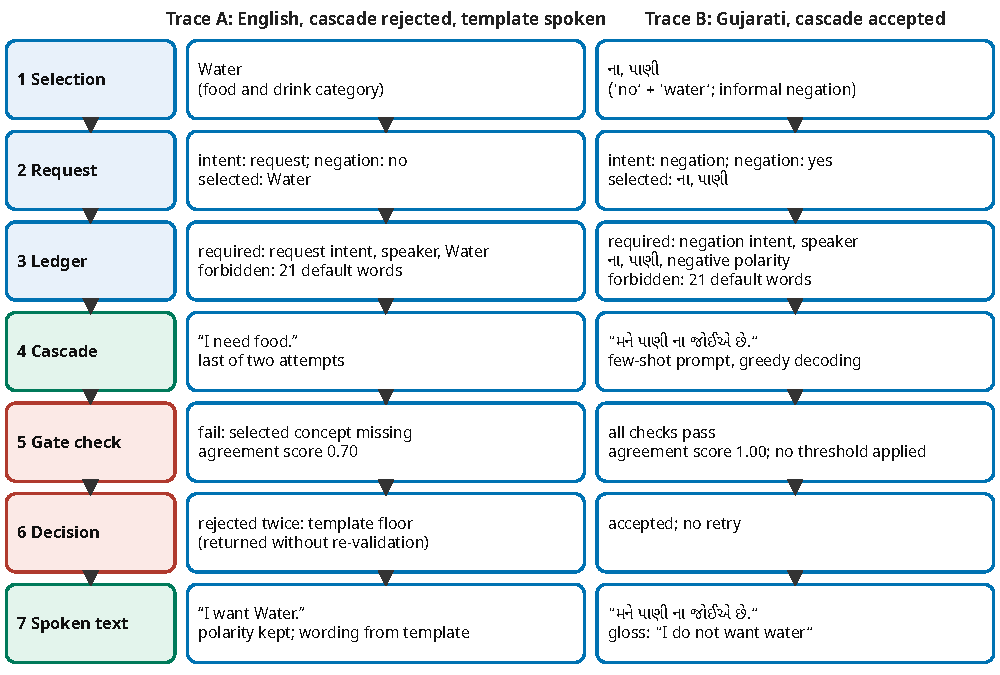
\includegraphics[width=\textwidth]{figures/workflow.pdf}
\caption{Interaction traces. Trace A: an English request whose cascade output is rejected twice and replaced by the template. Trace B: a Gujarati request whose cascade output is accepted; gloss: ``I do not want water'' (informal negation).}
\label{fig:workflow}
\end{figure*}

\section{Scorer Definitions and Scenario Families}
\label{app:scorer}
Retention is the share of required concept instances present (lexicon forms with inflection stems).
Polarity is correct when a negator is present exactly if the gold message is negated.
The act is correct when a request marker (want, need, \hi{चाहिए}, \gu{જોઈએ}, \hi{हवे}) or, for feelings, a feeling marker without a request marker is present.
A concept is \emph{added} if any other board concept or a time, meal, or venue word occurs.
An output is \emph{off-task} if it is a refusal, a third-person report (``the user\ldots''), empty, longer than 25 tokens, or contains Latin text in an Indic target.
Scenarios, lexicon, scorer, and raw outputs are in the release package; Table~\ref{tab:type} breaks success down by scenario family.
On the eight exploratory Hinglish scenarios the deployed pipeline succeeds on \CMSuccDepU{} (client) and \CMSuccDepS{} (explicit), the unconstrained prompt on \CMSuccNaive{}, and the template on \CMSuccTmplU{} and \CMSuccTmplS{}.

\begin{table}[t]
\centering\footnotesize
\setlength{\tabcolsep}{2.6pt}
\begin{tabular}{@{}lcccccc@{}}
\toprule
 & \multicolumn{3}{c}{Client payload} & \multicolumn{3}{c}{Explicit fields} \\
\cmidrule(lr){2-4}\cmidrule(l){5-7}
Scenario family ($n$) & Pre & Dep. & Tmpl & Pre & Dep. & Tmpl \\
\midrule
Food/drink request (35) & 26 & 29 & 35 & 26 & 29 & 35 \\
Refusal (\emph{No}+food) (38) & 19 & 33 & 38 & 10 & 38 & 38 \\
Feeling (30) & 3 & 4 & 5 & 18 & 22 & 30 \\
Negated feeling (32) & 2 & 1 & 0 & 2 & 13 & 24 \\
Action + object (24) & 8 & 18 & 24 & 8 & 18 & 24 \\
Help/call + person (16) & 7 & 12 & 16 & 7 & 12 & 16 \\
\midrule
All (175) & 65 & 97 & 118 & 71 & 132 & 167 \\
\bottomrule
\end{tabular}
\caption{Successful scenarios by family on the primary set. Pre: cascade before the gate; Dep.: deployed output; Tmpl: template floor.}
\label{tab:type}
\end{table}


\section{Trained Components}
\label{app:models}

Table~\ref{tab:models} lists the learned components.
Qwen2.5-0.5B-Instruct and IndicF5 are used as released.
\emph{Refiner.} The English refiner fine-tunes Flan-T5-small (76,961,152 parameters) to map selected concepts and an intent to one sentence, with 32-bit floating point, learning rate $10^{-4}$, weight decay 0.01, batch size 16 with two accumulation steps, 10 epochs (960 updates), seed 42, and one NVIDIA TITAN Xp (204\,s); the checkpoint with the lowest validation loss is kept.
Training, validation, and test hold 3,052, 384, and 384 template-generated payloads in 318, 40, and 40 disjoint groups; a fluency arm first adapts for 500 updates on 4,380 denoising pairs.
On the test payloads the fine-tuned model reaches \RefAModel{} exact match (\RefFModel{} with fluency pre-adaptation) and makes no negation error in 172 negated payloads, at a median of \RefALat{}\,ms; rules and the hybrid score \RefARules{} because references come from the same template families.

\begin{table*}[t]
\centering\footnotesize
\setlength{\tabcolsep}{3pt}
\begin{tabular}{@{}L{2.9cm}L{2.2cm}L{7.3cm}L{2.6cm}@{}}
\toprule
Component & Role in the demo & Training or adaptation & Data \\
\midrule
Qwen2.5-0.5B-Instruct (rev.\ 7ae5576) & realizer, refiner, verifier & Prompted, not fine-tuned (few-shot for HI, GU, MR) & -- \\
IndicF5 + Vocos & speech & Pretrained; zero-shot voice conditioning on a clip and its transcript & 1,417\,h, four corpora \\
HMM-1, HMM-2 & optional fallback prediction; Un-Jumble & Streamed in 500K-sentence chunks, pruned at counts 3 (4-grams) and 2 (trigrams). HMM-1: Jelinek--Mercer weights .50/.30/.15/.05. HMM-2: word and POS trigrams, exact search to 6 words, beam 64 above & English high-quality sentences, Tatoeba, Pile slices \\
Gutenberg HMM & English baseline & Bigram and trigram counts: 188,402 sentences; 63,783 bigram and 713,845 trigram states & public-domain books \\
Hindi AAC HMM & Hindi fallback & 3,867 turns, 2,171 word types (retrained on 3,078 training turns for evaluation) & Hindi dialogues \\
Suffix trie ($\infty$-gram) & primary next word & Count-based, built at start-up (\IGSent{} sentences, depth \IGDepth{}) & EN and HI dialogues \\
Flan-T5-small refiner & companion tool & Fine-tuned as described above & 3,052 template payloads \\
\bottomrule
\end{tabular}
\caption{Learned components, from the training records, run configurations, and model files in the release package. The IndicF5 corpora are Rasa, IndicTTS, LIMMITS, and IndicVoices-R.}
\label{tab:models}
\end{table*}


\end{document}
